\chapter{Lateral histograms}
This chapter treats of lateral histograms, which in our case simplify to row and column sums of the image. Although being very simple in principle, the lateral histograms show as a strong and robust method for EPOH and ECH detection. The largest part of its success, however, depends on the methods for estimating the period from the histograms. We present several such methods and their comparison.

\section{Lateral histograms applied to ionograms}
Lateral histograms are a little more general notion than we need in ionograms. We first provide the general definition and then we look for the more specialized one. We also observe a great simplification brought to this method by the nature of ionograms.

\subsection{Definition}
The general definition of lateral histograms is that ``the lateral histogram technique involves projecting an image on two or more axes by summing pixel intensities [\ldots] and using the resulting histograms to identify objects in the image.'' \citep{Davies2004} As can be seen, the title ``histograms'' does not have exactly the common meaning (counts of points with similar values). The slightly changed definition uses sums instead of counts and the ``similar values'' mean the same position with respect to the chosen axis.

To detect EPOHs and ECHs it is sufficient to take into account only the vertical and horizontal axes (whereas the definition allows for arbitrary axes). This is because EPOHs are strictly vertical lines and ECHs strictly horizontal. Summing up rows or columns, it can be clearly seen that in most cases the harmonic echoes generate high peaks in these histograms. The height of the peak corresponds to the length of the harmonic echo line as can be seen in Fig. \ref{fig:colSums}. 

\begin{figure}
	\centering
	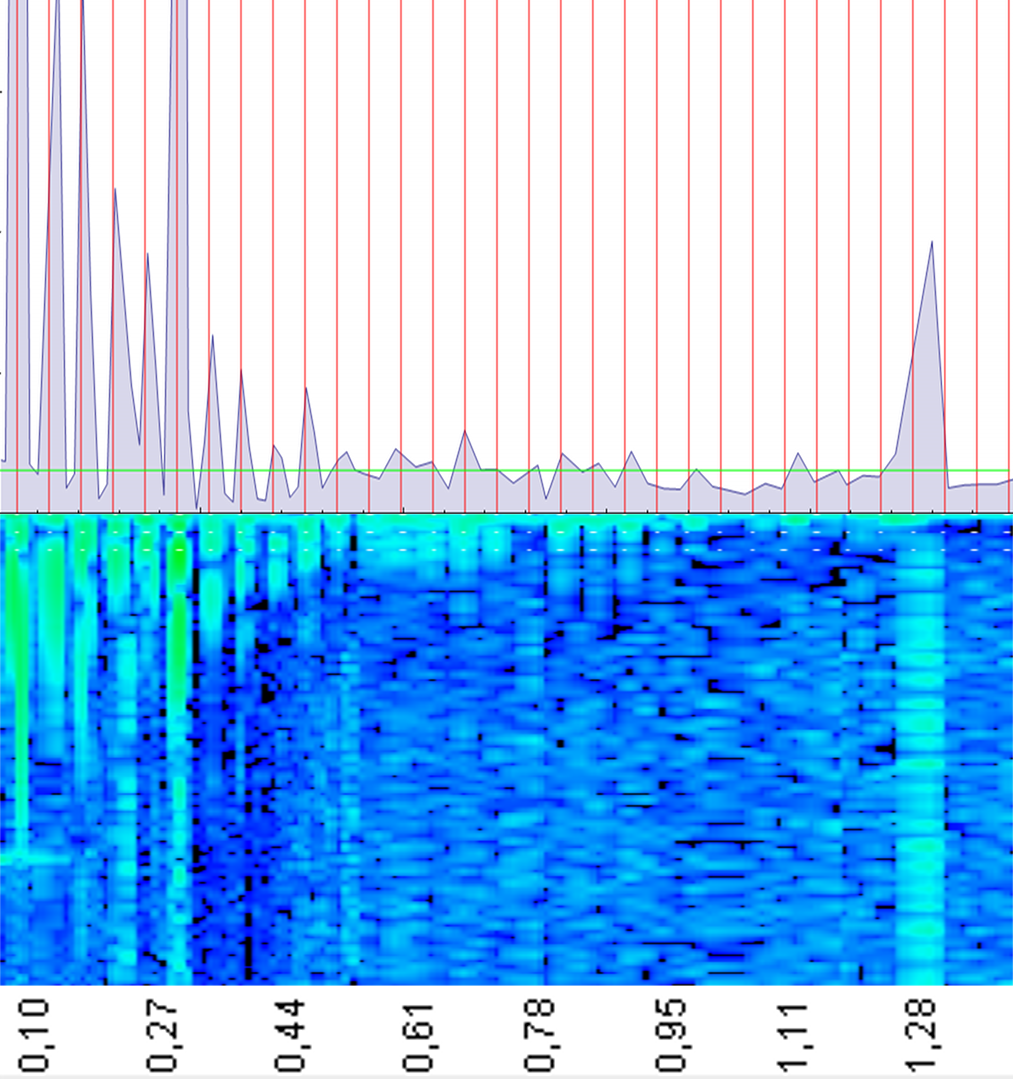
\includegraphics[width=140mm]{images/column_sums_orbit_3974_000.png}
	\caption{The column sums of a part of ionogram. The ionogram below is displayed along the sounding frequency scale in MHz. The top part shows the column sums at the frequencies from ionogram. The red lines represent the harmonics of the manually measured repetition period. They very closely correspond to the peaks in column sums. The green horizontal line denotes the mean value of the sums.}
	\label{fig:colSums}
\end{figure}

\subsection{Simplification in the case of ionograms}
The general definition assumes we are looking for point-like structures (given by 2~coordinates) and thus requires computing the histogram along at least two axes. From two histograms both 2D coordinates can be determined, but often there are ambiguities in the solution (for features overlapping in the direction perpendicular to an axis) \citep[chap.~13]{Davies2004}. The removal of such ambiguities is not trivial. 

Fortunately, in the ionogram case, only one axis is sufficient for every feature, since we are not interested in the length of the echo lines. Having the one histogram, detection of its peaks is all that is needed. Not all peaks in the histogram correspond to a harmonics line, some lower of them can be caused by noise. We call the peaks from harmonics lines ``real peaks'' and the others ``false peaks''.

\section{Implementation}
We implemented a feature detector using the lateral histograms technique on evenly sampled ionograms. It can be found on the attached CD in directory \texttt{programs/detector-summing}. See \nameref{sec:running} for information on how to run it. 

\subsection{Finding and filtering the peaks}
Due to the properties of both EPOH and ECH we can reduce the problem to working on the left half of ionograms. It may happen that some EPOHs stretch beyond the half, but in such cases there have to be lots of other harmonic lines in the left part (since the harmonics are the stronger the closer they are to the base frequency). As all ECHs start at the left border and usually are not very long, cutting the image in half is also possible.

As stated above, not all peaks in the histogram belong to the harmonic echoes. In order to find only the high peaks, we first filter out \n[\%]{50} of the row/column sums with the lowest values. We should be able to detect periods of length 2 bins, which would give just the \n[\%]{50} threshold. As can be derived from \citep[p.~3]{Akalin2010}, detecting periods less than \n{2.5} bins is impractical in the time domain, which yields threshold of \n[\%]{60}. As echoes in the frequency domain have to be sparser (due to the quasi-logarithmic spacing and quantization to bins), we can use this threshold, too.

With the uninteresting values filtered out (by setting them to zero) we can proceed to finding the peaks. The algorithm is rather simple, it just treats as a peak every data point with both neighboring values lower or equal to it. Once it finds a peak it zeroes out both non-increasing sequences neighboring to it (to get rid of non-strict maxima). What remains are the highest local maxima of the histogram.

\subsection{Determining the period}
In an ideal case the set would contain all the harmonic lines positions and no more. In practice, noise and data inaccuracies introduce some false peaks. As a heuristic to tell if a peak comes from harmonic lines, we can look at its height. The echo lines are often long and have their values more than 10~times higher than the background around them. Both these facts contribute to greater values of the row/column sums. For EPOH, if there are some ECH lines or an IE in the image, they disappear in the peaks list. It is because they are perpendicular to the EPOH lines and so may fill up the space between EPOHs, but in the frequency domain, their contribution is relatively small in comparison with the contribution of the EPOH lines. Ground echoes are almost completely discarded by cutting the ionogram in half. Similarly, while detecting ECH lines, the EPOH lines should cause no trouble. However, an IE can cause problems because it usually adds a very high and broad peak to row sums. This is a caveat of using this method to detect ECHs.

We should also be able to recognize when there are no data of interest in the ionogram. Using just row/column sums it would have been, however, more a statistical than algorithmic decision. We could say what levels of row/column sums mean no feature is present, or we could try to measure the ``ruggedness'' of the histogram to tell if there are some peaks, but we chose to rather not do such estimates and instead allow false positive detections. Removal of the false positives can be done later by comparing to the results of other methods more suitable to tell that a feature is not present at all. 

So we have the peaks and their heights as heuristics (telling us the probability of them to come from a line of interest). Combining these, we are finally able to estimate the repeat frequency. The last remaining task is to find a method taking peak positions and their weights and computing the most probable period. The following section lists three implemented methods.

\section{Period estimation}
A period estimation method has to count with the fact that there are some peaks missing and some of them are extra. It should hold that the extra peaks have relatively low weights. On the other hand, some ``regular'' peaks can also have low weights. Again, there is no absolute rule on the height of the peaks.

\subsection{Periodograms}
\label{ssec:periodogram}
The first proposed method is determination of the period from periodograms. Periodograms are defined in \citep{Scargle1982} for time series data. We slightly modify this definition to fit our purposes. Treat our set of peaks as a random variable $X$ measured at pixels $t_i$ along the axis (pixels without a peak yield zeros, the other ones). The measured values are denoted $\lbrace X_i = X(t_i): i = 1, 2, \ldots, N_0 \rbrace$. In our case, $N_0$ is the number of pixels along the axis. 

We first present a simple form of periodogram which is fundamental for understanding the principles behind periodograms. The periodogram of random variable $X$ at frequency $\omega$ is by \citep{Scargle1982} defined as: 
\begin{align}
P_X(\omega) &= \frac{1}{N_0} {\left| \sum\limits_{j=1}^{N_0} X(t_j) \exp(-\imath\omega t_j) \right|}^2 \\
&= \frac{1}{N_0} \left[ \left( \sum\limits_{j=1}^{N_0} X(t_j)\cos\omega t_j \right)^2 + \left(\sum\limits_{j=1}^{N_0} X(t_j)\sin\omega t_j  \right)^2 \right]
\label{eq:periodogramClassic}
\end{align}
The explanation of the meaning of this expression is ``that if X contains a sinusoidal component of frequency $\omega_0$, then at and near $\omega = \omega_0$ the factors $X(t)$ and $\exp(-\imath\omega t)$ are in phase and make a large contribution to the sums in equation \eqref{eq:periodogramClassic}. At other values of $\omega$ the terms in the sum are randomly positive and negative, and the resulting cancellation yields a small sum.'' \citep[p.~836]{Scargle1982} This means that there should be high distinctive peaks of $P_X$ near the $\omega$ values close to the frequency of the sinusoid. 

Another important fact is that it is sufficient to evaluate $P_X$ at a finite set of frequencies to get the correct one. This set is, according to \citep[p.~850]{Scargle1982}, as follows:
$$ \lbrace \omega_n = 2\pi n / N_0 \mid n = -N_0/2, \ldots, +N_0/2 \rbrace $$
The meaning of this set can be understood in this way: ``The fundamental frequency, $\omega_1 = 2\pi / N_0$, corresponds to a sine wave with frequency equal to the whole interval $N_0$. This is roughly the lowest frequency about which there is information in the data. The so-called Nyquist frequency, $\omega_N = \frac{1}{2}(2\pi/{\Delta t}) = \pi$ ($\Delta t = 1$ is the sampling of the interval) is roughly the highest frequency about which there is information, because $\Delta t$ is the shortest time interval spanned.'' \citep[pp.~850--851]{Scargle1982}.

Finally, we present a modified version of periodogram devised in \citep{Scargle1982}. The new definition has several benefits, but for us it is important that it is phase invariant (since we do not know the phase of the signal). The definition by \citep[p.~838]{Scargle1982} is the following:
\begin{align}
P_X(\omega) = \frac{1}{2} \left\lbrace \frac{\left[ \sum\limits_{j=1}^{N_0} X(t_j)\cos\omega (t_j - \tau) \right]^2}{\sum\limits_{j=1}^{N_0} \cos^2\omega (t_j - \tau)} + \frac{\left[\sum\limits_{j=1}^{N_0} X(t_j)\sin\omega (t_j - \tau) \right]^2}{\sum\limits_{j=1}^{N_0} \sin^2\omega (t_j - \tau)} \right\rbrace,
\label{eq:periodogramBetter}
\end{align} 
where $\tau$ can be computed from
\begin{align}
\tan(2\omega\tau) = \left. \left(\sum\limits_{j=0}^{N_0} \sin 2\omega t_j \right) \middle/ \left(\sum\limits_{j=0}^{N_0} \cos 2\omega t_j \right) \right.
\end{align} 
Summed up, $\tau$ is the term providing phase invariance. The form \eqref{eq:periodogramBetter} has also better statistical properties and can be used with uneven sampling (which we do not need)\citep[p.~849]{Scargle1982}.

Our implementation passes the list of peaks to the periodogram function $P_X$ and computes the periodogram for the $N_0$ frequencies $\omega_n$. Then it selects the highest peak and computes the period belonging to it. An example of the periodogram is shown in Fig. \ref{fig:periodogram}. Unfortunately, we have not found out how to incorporate peak weights to the algorithm. We tried multiplying every peak with its weight. Compared to the unweighted case, the results were even worse. We also tried to select the best peak among the 10~highest peaks (according to the mean of the column sums corresponding to the peaks). But the assessment method is probably not so strong, so in most cases the total result remains unchanged. 

\begin{figure}
	\centering
	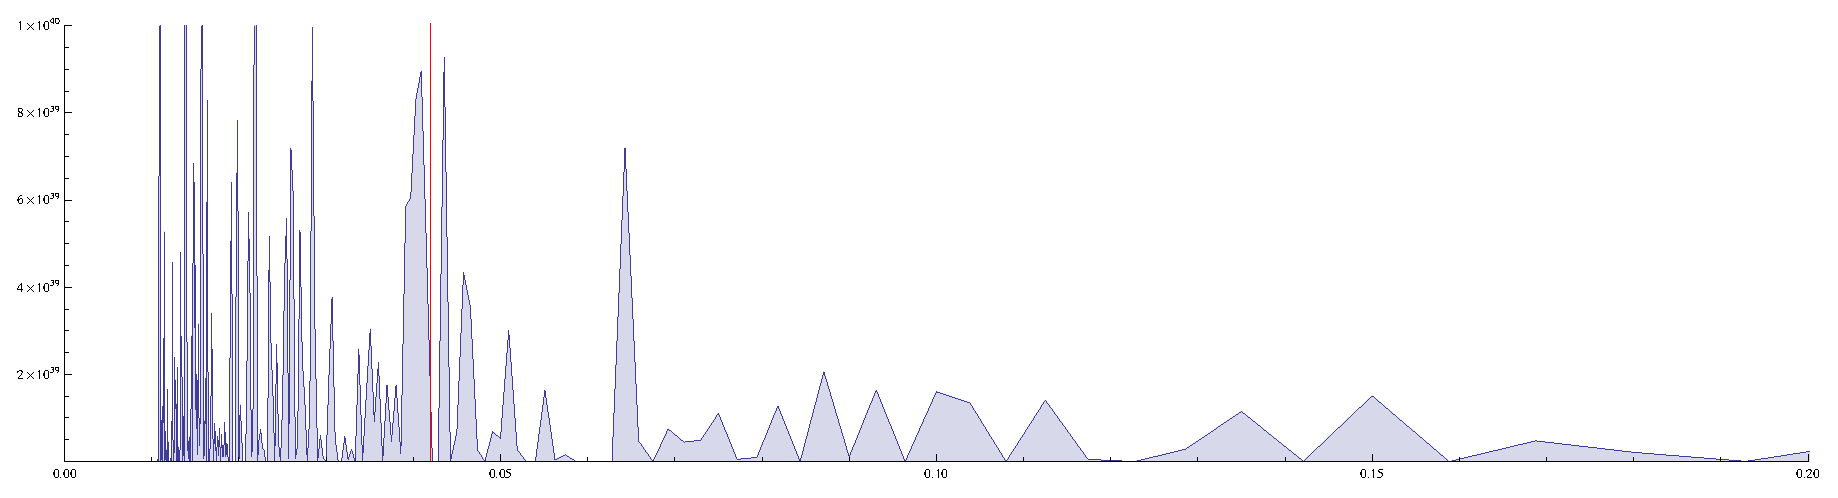
\includegraphics[width=140mm]{images/periodogram_from_normalized_peaks_orbit_3874_000.eps}
	\caption{The periodogram computed from the first ionogram in orbit 3874. The horizontal axis does not, however, show the frequency $\omega$ as is usual for periodograms, but it is already converted to correspond to the repetition period. The red vertical line is at the place of the manually measured repetiton frequency. It can be seen it tends to be near a large peak, but unfortunately at lower frequencies there are higher peaks that lead to incorrect results. The peaks in the left part are cropped at the top in order in interest of clarity.}
	\label{fig:periodogram}
\end{figure}
 
To assess the quality of the periodogram period estimation method, we perform two tests. In the first one we just measure the absolute difference between the estimated value and the manually acquired one; we denote it $E_A$. For simpler interpretation of the results we show the absolute error in ratio to the manually acquired value to get a percentage (for estimated period $p_e$ and manual period $p_m$ we compute~$E_A=|p_e-p_m|/p_m$). This is a nonuniform scaling, but it makes sense to require lower absolute errors for shorter periods.

We noticed that the estimated periods are often notable shorter than the target ones. After investigating the cause of this problem (which would render this method practically worthless) we found an explanation. Probably due to the (unweighted) false peaks the method tries to fit a sine wave which would go through all the real peaks as well as the false ones. This behavior makes the estimated periods be a ``1/integer'' fraction of the real period (eg. 1/2, 1/3, 1/4,~\ldots). This result looks interesting, because at least it allows us to considerably reduce the search space. Due to this property we also compute the second statistic $E_P$ (we call it the period corrected error) -- the error of the nearest integer multiple of the estimated period (that is $E_P=|[p_m/p_e]*p_e-p_m|/p_m$).

The results of these tests are shown in Figure \ref{fig:periodogram_errors}. As can be clearly seen, the absolute error $E_A$ with median \n[\%]{68} shows the results to be completely useless. On the other hand, the period corrected error with median \n[\%]{4.5} and \n{0.75}-quartile \n[\%]{7.6} looks like a relatively good result.   

\begin{figure}
	\centering
	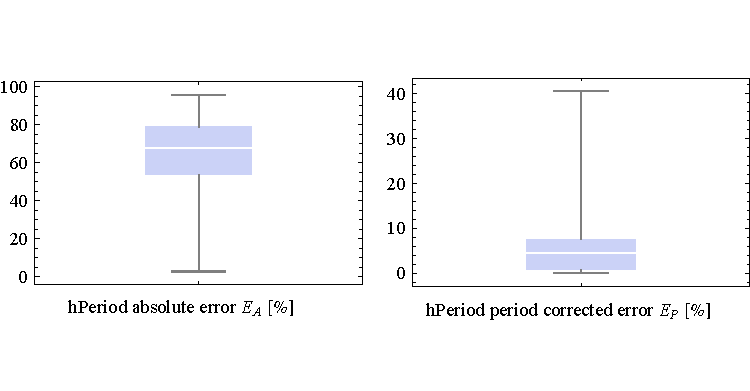
\includegraphics[width=140mm]{images/periodogram_errors.pdf}
	\caption{The errors of period estimation using the periodogram method. The tests were conducted on a set of ionograms from orbits 3836--4000. The left chart displays the absolute error $E_A$ with the \mbox{\n{0.25}-quartile}~=~\n[\%]{53}, median~=~\n[\%]{68} and the \mbox{\n{0.75}-quartile}~=~\n[\%]{79}. The right charts shows the period corrected error $E_P$ with the \mbox{\n{0.25}-quartile}~=~\n[\%]{0.8}, median~=~\n[\%]{4.5} and \mbox{\n{0.75}-quartile}~=~\n[\%]{7.6}.}
	\label{fig:periodogram_errors}
\end{figure}

To sum it up, the periodogram-based period estimation is not perfect for our task. On the other hand, its results can be utilized by other methods to scale down the search space. One more drawback is it only searches a fixed set of periods to try out.

\subsection{Sine wave fitting}
 
\section{Ground echo detection}















